\def\year{2017}\relax %\typeout{Probabilistic Alternating-Time $\mu$-Calculus}
\documentclass[letterpaper]{article}
%-----------------------------------------------------
\usepackage{aaai16}
\usepackage{times}
\usepackage{helvet}
\usepackage{courier}
\frenchspacing
\setlength{\pdfpagewidth}{8.5in}
\setlength{\pdfpageheight}{11in}

\pdfinfo{
/Title (Probabilistic Alternating-Time $\mu$-Calculus)
/Author (Fu Song) }
\setcounter{secnumdepth}{1}


\usepackage{amsmath}
\usepackage{amssymb}
\usepackage{amsthm}
\usepackage{mathrsfs}
\usepackage{wasysym}
\usepackage{color}
\usepackage{xspace}
\usepackage{txfonts}
\usepackage{graphicx}
\usepackage{enumerate}
\usepackage{tikz}
\usepackage{nicefrac}
\usepackage[ruled,linesnumbered]{algorithm2e}

%\usepackage{hyperref}
\frenchspacing
%-----------------------------------------------------

\newcommand{\AP}{{\bf AP}}
\newcommand{\calZ}{\mathcal{Z}}
\newcommand{\calM}{\mathcal{G}}
\newcommand{\calD}{\mathcal{D}}
\newcommand{\calF}{\mathcal{F}}
\newcommand{\calP}{{\sf Paths}}
\newcommand{\calT}{{\sf Tracks}}
\newcommand{\Ag}{\textsf{Ag}}
\newcommand{\Enc}{\textsf{enc}}
\newcommand{\Act}{\textsf{Act}}
\newcommand{\ND}{\textsf{ND}}
\newcommand{\Cycl}{\textsf{Cycl}}
\newcommand{\outcomes}{\textsf{Outcomes}}
\newcommand{\Prb}{\textsf{Pr}}
\newcommand{\nat}{\mathbb{N}}
\newcommand{\eval}{\textsf{eval}}
\newcommand{\nA}{\overline{A}}
\newcommand{\calS}{\mathcal{S}}

\newcommand{\PA}{\mathcal{P}}
\newcommand{\dec}{{\bf d}}
\newcommand{\pamc}{{pAMC}\xspace}
\newcommand{\pamcs}{{pAMC$_0$}\xspace}
\newcommand{\pamcc}{{pAMC$_1$}\xspace}
\newcommand{\pmutl}{{P$\mu$TL}\xspace}

\newcommand{\Nn}{\mathbb{N}}
\newcommand{\inff}{\textsf{inf}}
\newcommand{\opX}{{\bf X}}
\newcommand{\opW}{{\bf W}}
\newcommand{\opMax}{{\bf \lozenge}}
\newcommand{\opMin}{{\bf \square}}
\newcommand{\opU}{{\bf U}}
\newcommand{\opR}{{\bf R}}
\newcommand{\opG}{{\bf G}}
\newcommand{\opA}[1]{\langle{#1}\rangle}
\newcommand{\opUA}[1]{[{#1}]}

\newcommand {\semantics}[1]{\|{#1}\|}  %{\llbracket{#1}\rrbracket}

\newtheorem{example}{Example}
\newtheorem{remark}{Remark}
\newtheorem{definition}{Definition}
\newtheorem{theorem}{Theorem}
\newtheorem{lemma}{Lemma}
\newtheorem{proposition}{Proposition}


\newcommand{\authorComment}[3]
 {{\color{#1}\textbf{[\!\![\!\![\marginpar{\centering{\color{#1}\textbf{#2}}}~ #3 ]\!\!]\!\!]}}}
\newcommand{\ww}[1]{\authorComment{red}{WW}{#1}}
\newcommand{\fu}[1]{\authorComment{blue}{SF}{#1}}
\newcommand{\lj}[1]{\authorComment{purple}{LJ}{#1}}

%------------------------------------------------------
\begin{document}
%%
\title{Probabilistic Alternating-Time $\mu$-Calculus}
 \author{%Fu Song
        %\\East China Normal University, Shanghai, P. R. China\\
        %ShanghaiTech University, Shanghai, P. R. China
    %    \And
    %    Wanwei Liu
    %    \\ School of Computer Science, \\ National University of Defense Technology,\\ Changsha, P. R. China
    %    \And
    %    Lijun Zhang
    %    \\ State Key Lab. of Computer Science, \\       Institute of Software, CAS,\\ Beijing, P. R. China
 }
% \setlength\titlebox{2.7in}

\maketitle

%-----------------------------------------------------------
\begin{abstract}
In this paper, we propose \emph{probabilistic alternating-time $\mu$-calculus} (\pamc), a \emph{probabilistic} extension of the alternating-time temporal logic AMC, for expressing properties of multi-agent systems with uncertain behaviors.
The semantics of \pamc formulae is defined on \emph{probabilistic concurrent game structures} (pCGSs), which are a natural model of multi-agent systems with uncertain behaviors. We investigate the model-check problem of pCGSs against \pamc and two useful fragments \pamcc and \pamcs thereof.
We give a {\sc 2NExpTime} algorithm
for \pamc under memoryful setting and {\sc 2ExpTime} algorithm for \pamc under deterministic memoryless setting.
The problem for \pamcc is in $({\sc UP\cap co{-}UP})^{{\sc NP\cap co{-}NP}}$ under randomized memoryful setting and
deterministic memoryless setting.
For \pamcs, the problem is in ${\sc UP\cap co{-}UP}$ and tractable under randomized memoryful setting when the alternation depth is fixed.
\end{abstract}



%-----------------------------------------------------------
\section{Introduction}
\label{sec:intr}

%Multi-agent systems are being a new paradigm for robust and scalable software systems, in which autonomous agents can complete their objectives while %situated in a dynamic and uncertain environment. Therefore, it is significantly important to automatically and accurately analyze
%multi-agent systems. In this work, we propose \emph{probabilistic alternating-time $\mu$-calculus} (\pamc), a probabilistic extension of the alternating-time temporal logic AMC, for expressing probabilistic properties of multi-agent systems. \pamc is strong enough to encode
%probabilistic alternating-time temporal logic pATL$^*$ and AMC.
%Semantics of \pamc formulae are defined with respect to \emph{probabilistic concurrent game structures} (pCGSs), which are a natural model of multi-agent %systems with uncertain behaviors. We investigate the model-check problem of pCGSs against \pamc and thereof useful fragments \pamcc and \pamcs, as well %as the memorability and determinacy problems of strategies of agents to fulfill the properties.
%We show that \pamcc has memoryless property, but \pamc does not. On the other hand, \pamc has determinacy property.
%For the model-checking problem, we given a {\bf 3EXPTIME}algorithm
%for \pamc under randomized or deterministic memoryful setting and {\bf 2EXPTIME} algorithms for \pamc and \pamcc under deterministic memoryless setting %and randomized memoryful setting respectively. Under deterministic memoryless setting, we show that the problem for \pamcc is in {\bf EXPTIME}.
%For \pamcs, the problem is in ${\bf UP\cap co{-}UP}$ and can be decided in polynomial time under randomized memoryful setting when the alternation depth %is fixed.


A \emph{multi-agent system} (MAS), in a nutshell, is a computerized system composed of autonomous agents, in which the
behavior of each agent is determined by its observed information of the system.
MASs have been successfully used to solve problems that are difficult or inefficient for an individual agent to
tackle. However, the coexistence of multiple autonomous agents in a MAS makes
it significantly difficult to precisely analyze the system behaviors.

\emph{Model-checking} that exhaustively and automatically checks whether a model meets a given specification, has been extended to MASs \cite{AHK02}.
In \cite{AHK02}, MASs are modeled as \emph{concurrent game structures} (CGSs) and specifications are expressed in \emph{alternating-time temporal logics}, e.g., ATL, ATL$^*$ and alternating-time $\mu$-calculus (AMC), for which model checking algorithms were also given therein and later implemented in the model-checker MOCHA \cite{AHMQRT98}.
Starting from these works, both the formal methods community and the AI community have placed increasing emphasis on model-checking MASs including specification logics, MAS models and their model-checking algorithms.
Many extension of alternating-time temporal logics were introduced, as well as variants of MAS models.


For reasoning about agents' knowledge, or belief, desire and intention, extensions of ATL with \emph{knowledge operators} \cite{HkW02} and
\emph{belief, desire, and intention operators} were proposed \cite{BB05}, in which the CGSs are extended with \emph{accessibility relations}.
To express cooperation and enforcement of agents, a more expressive logic, called \emph{strategy logic}, was proposed in \cite{MMV10}.
Generally, its model-checking problem is undecidable. Therefore, several decidable fragments of strategy logic were investigated \cite{CLM15,MMS13,MMS14,MMPV14}.
\cite{HP06,BLMO07} investigated timed alternating-time temporal logics and timed CGSs to reason about timed world.


In order to make accurate analysis of more complex multi-agent systems in which agents (e.g., environment) may have random or uncertain behaviors due to unpredictable physical
conditions,  Chen and Lu extended CGSs, ATL and ATL$^*$ with \emph{probability} leading to \emph{probabilistic CGSs} (pCGSs), \emph{pATL} and \emph{pATL$^*$} \cite{CL07a}.
Later, Chen et al. proposed an extension of pATL with \emph{reward operators}. These techniques were implemented in a model-checker {PRISM}-games which were successfully applied to analyze probabilistic MASs \cite{CFKPS12,CFKPS13b}. Schnoor studied the bisimulations contained in pATL$^*$ and the complexity of the model-checking problem under incomplete information (i.e., agents can only observe partial information of  systems) and memoryless (i.e., decision made by agents only depend on the last state rather than the full history) setting \cite{Sch10}.
Huang et al. investigated the pATL$^*$ model-checking problem over probabilistic interpreted systems with incomplete
information and synchronous perfect recall \cite{HSZ12}. Unfortunately, this problem is undecidable.


Besides these works, it is worth to mention the work on \emph{pushdown multi-agent systems} which can model \emph{infinite-state} multi-agent systems \cite{MP15}.
The model-checking problems of pushdown multi-agent systems against alternating-time temporal logics (such as ATL, ATL$^*$ and AMC) and variant fragments of strategy logic were studied in
\cite{MP15,CSW16a,CSW16b}.


This paper follows the direction of \cite{CL07a}. We introduce \emph{probabilistic alternating-time $\mu$-calculus} (\pamc) which can been seen as an \emph{probabilistic} extension of AMC or an \emph{alternating-time} generalization of probabilistic $\mu$-calculus \cite{CKP15}.
The semantics of \pamc is defined over pCGSs in which strategies of agents and transition functions are respectively equipped with probability distribution on decisions and successor states. \pamc can express interesting properties that cannot be expressed by pATL$^*$. For example, let us consider the following property:
\begin{quote}
Agents $1$ and $2$ have strategies such that whatever other agents do, the probability of occurrence of $p$ at every even position is greater than 0.9.
\end{quote}
This property cannot be expressed by any pATL$^*$ formula, but can be expressed in \pamc as the formula $\opA{\{1,2\}}^{> 0.9}\nu Z.(p\wedge \opX \opX \ Z)$.


We investigate memorability, determinacy and model-checking problems for \pamc, as well as its two fragments: \pamcs and \pamcc. \pamcs and \pamcc are obtained by restricting syntax of \emph{path formulae} in \pamc.
\pamc is strictly more expressive than AMC and pATL$^*$ \cite{CL07a} and is able to encode several well known logics such as P$\mu$TL,  pCTL, pCTL$^*$ and probabilistic $\mu$-calculus for one-agent pCGSs (i.e., Markov decision processes) \cite{LSWZ15,CKP15}.
In addition, \pamcs and \pamcc are able to encode AMC and pATL, respectively.
We obtain several interesting results. In particular,  \pamc does not have memoryless property, but \pamcc has.
\pamc enjoys determinacy property under memoryful setting which will lose if only memoryless strategies are allowed.

Concerning on the model-checking problem, we show that the problem for \pamc is in {\sc 2NExpTime} under randomized/deterministic memoryful setting and in {\sc 2ExpTime} under deterministic memoryless setting.
For \pamcc, the problem
is in $({\sc UP\cap co{-}UP})^{{\sc NP\cap co{-}NP}}$ under randomized memoryful setting and
deterministic memoryless setting. For \pamcs, the problem is in ${\sc UP\cap co{-}UP}$ and can be decided in polynomial time
of the size of pCGSs.


Due to lack of space, the discussion of expressiveness with respect to AMC \cite{AHK02}, pATL$^*$ \cite{CL07a} and $\mu$-pCTL \cite{CKP15}, and the proofs for memorability and determinacy are given in the supplemental material.


%----------------------------------------------------------------
\section{Concurrent Games}
We fix a countable set $\AP$ of \emph{atomic propositions}.
Let $[k]$ denote the set $\{1,...,k\}$ for a given natural number $k\in \nat$.
For a countable set $X$, a \emph{probability distribution} on $X$
is a function $\Prb:X\rightarrow[0,1]$ such that $\sum_{x\in X}\Prb(x)=1$.  Let $\Upsilon(X)$ denote the set of probability distributions on $X$.
A \emph{$\sigma$-algebra} over a set $\Omega$ is a subset $\calF\subseteq 2^\Omega$ such that $\calF$ is closed under complement and countable union, in which each element of $\calF$ is called an \emph{event}.
A \emph{probability space} is a triple $(\Omega,\calF, \Prb)$, where $\Omega$ is a \emph{sample space}, $\calF\subseteq \Omega$ is a $\sigma$-algebra over $\Omega$, $\Prb:\calF\rightarrow[0,1]$ is a
\emph{probability measure} such that $\Prb(\Omega)=1$ and for each two disjoint events $X,Y\in \calF$, $\Prb(X\cup Y)=\Prb(X)+\Prb(Y)$.



\subsection{Probabilistic Concurrent Game Structures}
\begin{definition}[Probabilistic Concurrent Game Structures]
A \emph{probabilistic concurrent game structure} (pCGS) is a tuple $\calM=(\Ag,\Act, Q, \delta,\lambda,q_0)$, where
\begin{itemize}
  \item $\Ag=\{1,...,n\}$ is a finite set of \emph{agents} (a.k.a. players),
  \item $\Act$ is a finite set of \emph{actions} which can be made by agents, we use $\calD$ to denote the set of \emph{decisions} $\dec=\langle a_1,...,a_n\rangle$ such that $\forall i\in [n], a_i\in \Act$, denoted by $\dec(i)$, is the action made by the agent $i$,
  \item $Q$ is a finite set of \emph{states} with $q_0\in Q$ as the initial state,
  \item $\delta:Q\times \calD\times Q\rightarrow [0,1]$ is a \emph{probability transition function} such that for every $q\in Q,\dec\in\calD$, $\sum_{q'\in Q}\delta(q,\dec,q')=1$,
  \item $\lambda:\AP\rightarrow 2^{Q}$ is the \emph{labelling function} assigning to each atomic proposition a set of states.
\end{itemize}
\end{definition}

Given two states $q_1,q_2\in Q$, $q_2$ is a \emph{possible successor} of $q_1$ if there exists a decision $\dec\in\calD$ such that $\delta(q_1,\dec,q_2)>0$.
Intuitively, if $\delta(q_1,\dec,q_2)>0$ and the pCGS $\calM$ is at the state $q_1$, then the agents $\Ag$ in the pCGS $\calM$ can make the decision $\dec$ such that $\calM$ moves from the state $q_1$ to the state $q_2$
with probability $\delta(q_1,\dec,q_2)$.

A \emph{track} $\pi\in Q^+$ is a finite sequence of states $q_0q_1...q_m$ such that for every $i\in[m]$, $q_i$ is a possible successor of $q_{i-1}$. Given a track $\pi=q_0q_1...q_m$, for every $i\in\{0,...,m\}$, we use $\pi_i$ to denote the state $q_i$, $\pi_{\geq i}$ to denote the suffix $q_iq_{i+1}...q_m$, and $\pi_{\leq i}$ to denote the prefix $q_0...q_{i}$.
Let $\calT_\calM=Q^+$ denote the set of all the possible tracks
of $\calM$ and $\calT_{\calM,q}$ denote the set of all the possible tracks that start from the state $q\in Q$.

A \emph{path} $\rho\in Q^\omega$ is an infinite sequence of states $q_0q_1...$ such that for every $i\geq 1$, $q_i$ is a possible successor of $q_{i-1}$. Similarly, we use $\rho_i$ to denote the state $q_i$, $\rho_{\geq i}$ to denote the suffix $q_iq_{i+1}...$, and $\rho_{\leq i}$ to denote the prefix $q_0...q_{i}$.
Let $\calP_\calM=Q^\omega$ denote the set of all the possible paths
of $\calM$ and $\calP_{\calM,q}$ denote the set of all the possible paths that start from the state $q\in Q$.
Whenever $\calM$ is clear from the context,  $\calT_{\calM}$, $\calT_{\calM,q}$, $\calP_{\calM}$ and $\calP_{\calM,q}$ are abbreviated as $\calT$, $\calT_{q}$, $\calP$ and $\calP_{q}$ respectively.

%A pCGS $\calM=(\Ag,\Act, Q, \delta,\lambda,q_0)$  is a \emph{concurrent game structure} (CGS)
%if for every $\delta:Q\times \calD\times Q\rightarrow \{0,1\}$.

\subsection{Strategies and Probability Measure of pCGSs}
A \emph{randomized strategy} for an agent $i\in\Ag$ in the pCGS $\calM$ is a function $\theta:\calT\rightarrow \Upsilon(\Act)$ that assigns to each track (i.e., the history the agent saw so far) a probability distribution on $\Act$. A randomized strategy $\theta:\calT\rightarrow \Upsilon(\Act)$ is \emph{deterministic} if for every track $\pi\in\calT$, there is only one action $a\in\Act$ such that $\theta(\pi)(a)=1$ (hence $\theta(\pi)(a')=0$ for any other action $a'$).
A randomized/deterministic strategy $\theta:\calT\rightarrow \Upsilon(\Act)$ is \emph{memoryless} if for every $\pi,\pi'\in\calT$ and $q\in Q$, $\theta(\pi q)=\theta(\pi' q)$, otherwise is \emph{memoryful}. Memoryless strategy can be simplified as a function $\theta:Q\rightarrow \Upsilon(\Act)$.
%Given a track $\pi\in\calT$ and a decision $\dec\in\calD$, let $\Prb^{\upsilon_A,\upsilon_{\nA}}(\pi,\dec)=\prod_{j\in A}\upsilon_A(j)(\pi)(\dec(j)) %\cdot \prod_{j\in \nA} \upsilon_{\nA}(j)(\pi)\dec(j)$ denote the possibility
%of the decision $d$ made by the agents under the track $\pi$.
Let $\Theta$ denote the set of all the possible strategies.

A \emph{coalition} is a set of agents $A\subseteq \Ag$, a \emph{coalition strategy} of $A$
is a function $\upsilon_A: A \rightarrow \Theta$ that assigns to each agent $i\in A$ a strategy $\upsilon_A(i)$.
We use $\nA$ to denote the set of agents $\Ag\setminus A$. A \emph{response strategy} of $A$ is a function $\upsilon_{\nA}: \nA \rightarrow \Theta$ which assigns to each agent $i\in\nA$ (i.e., agent $i$ out of $A$) a strategy $\upsilon_{\nA}(i)$.
Let $V_A$ and $V_{\nA}$ respectively denote the sets of all the possible coalition strategies and response strategies of $A$.
Given a track $\pi$, a decision $\dec\in\calD$, a coalition strategy $\upsilon_A$ and a response strategy $\upsilon_{\nA}$ of $A$,
let $\Prb^{\upsilon_A,\upsilon_{\nA}}(\pi,\dec)$ denote the probability:
\[\prod_{i\in A}\upsilon_A(i)(\pi)(\dec(i))\cdot \prod_{i\in \nA}\upsilon_{\nA}(i)(\pi)(\dec(i)),\]
that is the probability of the decision $\dec$ made by the agents $\Ag$ with respect to the track $\pi$.

Given a coalition $A\subseteq\Ag$, a coalition strategy $\upsilon_A$ and a response strategy $\upsilon_{\nA}$ of $A$,
a path $\rho$ is \emph{compatible} with the coalition strategy $\upsilon_A$ and the response strategy $\upsilon_{\nA}$, if the following conditions hold:
\begin{itemize}
  \item for every $i\geq 0$, there is a decision $\dec_i\in \calD$ such that $\delta(\rho_i,\dec_i,\rho_{i+1})>0$,
  \item $\upsilon_A(j)(\rho_{\leq i})(\dec_i(j))>0$ for all $j\in A$,
  \item $\upsilon_{\nA}(j)(\rho_{\leq i})(\dec_i(j))>0$ for all $j\in \nA$.
\end{itemize}
Intuitively, the compatible condition of paths rule out infeasible paths under the coalition strategy $\upsilon_A$ and the response strategy $\upsilon_{\nA}$.

Let $\calP_q^{\upsilon_A,\upsilon_{\nA}}$
denote the set of paths starting from $q$ that are compatible with respect to $\upsilon_A$ and $\upsilon_{\nA}$.
Formally, \[\calP_q^{\upsilon_A,\upsilon_{\nA}}=\{ \ \rho\in \calP_q \mid \rho \mbox{ is compatible with } \upsilon_A \mbox{ and } \upsilon_{\nA} \ \}.\]

Given the coalition strategy $\upsilon_A$ and response strategy $\upsilon_{\nA}$ of the agents $A$, a \emph{cyclinder set} (i.e., \emph{event}) of a track $\pi$ is defined as the set:
\[\Cycl^{\upsilon_A,\upsilon_{\nA}}(\pi) \ = \ \{ \ \rho\in \calP_{\pi_0}^{\upsilon_A,\upsilon_{\nA}}\mid \pi \mbox{ is a prefix of }\rho \ \}.\]
Let $\Cycl_q^{\upsilon_A,\upsilon_{\nA}}$ denote the set of cyclinder sets $\Cycl^{\upsilon_A,\upsilon_{\nA}}(\pi)$, where $\pi\in \calT_q$.
Given a coalition strategy $\upsilon_A$,  a response strategy $\upsilon_{\nA}$ and a state $q\in Q$, the probability space associated with the pCGS $\calM$ is the triple
$(\calP_q^{\upsilon_A,\upsilon_{\nA}}, \Cycl_q^{\upsilon_A,\upsilon_{\nA}}, \Prb_q^{\upsilon_A,\upsilon_{\nA}})$,
where the probability measure $\Prb_q^{\upsilon_A,\upsilon_{\nA}}$ is defined as: $\Prb_q^{\upsilon_A,\upsilon_{\nA}}\big(\Cycl^{\upsilon_A,\upsilon_{\nA}}(q)\big)=1$, and
$\Prb_q^{\upsilon_A,\upsilon_{\nA}}\big(\Cycl^{\upsilon_A,\upsilon_{\nA}}(q_0q_1...q_m)\big)=$
\[\prod_{i=0}^{m-1} \sum_{\dec\in\calD} \Prb_q^{\upsilon_A,\upsilon_{\nA}}(q_0q_1...q_i,\dec)\cdot \delta(q_{i},\dec,q_{i+1}),\]
where $q_0=q$. Notice that $\Cycl^{\upsilon_A,\upsilon_{\nA}}(q)=\calP_q^{\upsilon_A,\upsilon_{\nA}}$.



\subsection{Stochastic Parity Games}
Stochastic parity games are two-player turn-based concurrent games. We review stochastic parity games which will be used in our techniques.

\begin{definition}[Stochastic Parity Games]
A \emph{stochastic parity game} is a tuple $\calM=(V,E,(V_0,V_1,V_2),F,\Delta)$, where $(V,E)$ is a directed graph and $(V_0,V_1,V_2)$ is a partition of the set $V$ of vertexes,
$F:V\rightarrow\{0,...,k\}$ is a \emph{rank function}, and $\Delta:V_2\rightarrow\Upsilon(V)$ is a \emph{probabilistic transition function}.
\end{definition}
The vertexes in $V$ are called \emph{states},  in $V_0$ are called \emph{player-0 states}, in $V_1$ are called \emph{player-1 states} and
in $V_2$ are called \emph{probabilistic states}. Tracks and paths of stochastic parity games are defined similar to pCGSs. Given a path $\rho$, let $\inff(\rho)$ denote the set of infinite often visited states in $\rho$.
A \emph{strategy}  for player-i for $i\in\{0,1\}$ is a function $\theta:V^*V_i\rightarrow \Upsilon(V)$ that assigns to every track ending with a state in $V_i$ a distribution on states $V$. Let $\Theta_i$ with $i\in\{0,1\}$ denote the set of all strategies for player-i.
Given two strategies $\theta_0\in\Theta_0$ and $\theta_1\in\Theta_1$, the path $\rho$ is \emph{$(\theta_0,\theta_1)$-possible} for the game $\calM$ if for every $k\geq 0$ the following conditions hold:
if $\rho_k\in V_i$ for $i\in\{0,1\}$, then $\theta_i(\rho_{\leq k},\rho_{k+1})>0$, and if $\rho_k\in V_3$, then $\delta(\rho_{k},\rho_{k+1})>0$.
Given a state $v$, let $\outcomes(v,\theta_0,\theta_1)$ denote the set of  $(\theta_0,\theta_1)$-possible paths starting from $v$.
Similar to pCGSs, the strategies $\theta_0,\theta_1$ and the state $v\in V$ induce a probability space
$(\outcomes(v,\theta_0)(\theta_1), \Cycl_v^{\theta_0,\theta_1}, \Prb_v^{\theta_0,\theta_1})$ (details refer to \cite{CH12}).

A \emph{Markov chain} is a special case of stochastic parity game $\calM=(V,E,(V_0,V_1,V_2),F,\Delta)$ in which $V_0=V_1=\emptyset$.



Given a state $v$ and a number $r\in[0,1]$, player-0 \emph{wins} the game from the state $v$ with respect to a condition $\sim r$ if there exists a strategy $\theta_0\in\Theta_0$ such that for all $\theta_1\in\Theta_1$, the following condition holds: where $\sim\in\{\geq, >\}$, \[\Prb_v^{\theta_0,\theta_1}(\{\rho\in \outcomes(v,\theta_0,\theta_1)\mid \min\limits_{v'\in \inff(\rho)}F(v') \mbox{ is \emph{even}}\})\sim r.\]
The winning for player-1 is defined analogously.
Memoryless, memoryful, randomized and deterministic strategies in stochastic parity games are defined similar to
pCGSs.

\begin{theorem}
\label{thm-spg}\cite{CJH04,CH12}
Given a stochastic parity game $\calM$, a state $v$ and a condition $\sim r$, whether player-i for $i\in\{0,1\}$ can win the game or not can be decided in ${\sc NP\cap co{-}NP}$ or exponential time. The problem can be decided in polynomial time for Markov chain.
Moreover, deterministic memoryless strategies are sufficient to determine the problem.
\end{theorem}


\section{Probabilistic Alternating-Time $\mu$-Calculus}
In this section, we introduce \emph{probabilistic alternating-time $\mu$-calculus} (\pamc), a \emph{probabilistic} extension of AMC \cite{AHK02}.
In \pamc, we introduce two types of least and greatest fixpoints for state and path formulae, namely,
$\mu$ and $\nu$ are fixpoint operators for state formulae, and $\mu_p$ and $\nu_p$ are fixpoint operators for path formulae.
Existential and universal coalition quantifiers $\opA{A}$, $\opUA{A}$ are equipped with probabilistic constraints $\sim c$ for $\sim\in\{\geq, >\}$
and $c\in[0,1]$.


\begin{definition}[Probabilistic Alternating-Time $\mu$-Calculus]
Formally, let $\calZ$ be a finite set of proposition variables. The syntax of probabilistic alternating-time $\mu$-calculus (\pamc for short) formulae is depicted as follows: where
$\Phi$ are \emph{state formulae}, $\Psi$ are \emph{path formulae},
 \[\begin{array}{ll}
\Phi::= &p\mid  \ \neg p \mid  \ Z \ \mid \Phi \wedge \Phi  \ \mid  \ \Phi \vee \Phi \ \mid \\
& \mu Z. \Phi  \ \mid \ \nu Z. \Phi  \  \mid \ \opUA{A}^{\sim c} \Psi  \ \mid \   \opA{A}^{\sim c} \Psi\\\\
\Psi::=&\Phi \ \mid \Psi \wedge \Psi  \ \mid  \ \Psi \vee \Psi \ \mid \  \mu_p Z. \Psi  \ \mid \  \nu_p Z. \Psi \ \mid \ \opX \Psi
 \end{array}\]
where $p\in\AP$, $Z\in \calZ$, $c\in[0,1]$, $\sim\in\{\geq,>\}$ and  $A\subseteq \Ag$.
\end{definition}

A \pamc formula $\phi$ is \emph{closed} if each variable $Z\in \calZ$ used in $\phi$ is bound in the scope of a fixpoint operator $\mu Z$, $\nu Z$, $\mu_p Z$ or $\nu_p Z$.
A \pamc formula is called  a \emph{principal formula} $\phi$ if it is in the form of $\opUA{A}^{\sim c} \psi$ or $\opA{A}^{\sim c} \psi$, and no subformula of $\psi$
is in the form of $\opUA{A'}^{\sim' c'} \psi'$ or $\opA{A'}^{\sim' c'} \psi'$.
The \emph{alternation depth} of a formula $\phi$, denoted by $dep(\phi)$, is the number of alternations in the nesting of least and greatest fixpoints.
Let $\Ag^\phi$ denote the set of agents appeared in the formula $\phi$ and $true \equiv p\vee \neg p$ for $p\in\AP$.


The semantics of \pamc state formulae $\phi$ is given w.r.t. a pCGS and a valuation $\xi:\calZ\rightarrow 2^Q$.
We use $\xi[Z\mapsto S]$ to denote the valuation which is equal to $\xi$ except for $\xi[Z\mapsto S](Z)=S$.
Given a pCGS $\calM=(\Ag,\Act, Q, \delta,\lambda,q_0)$ and a valuation $\xi:\calZ\rightarrow 2^Q$,
the denotation function $\semantics{\circ}_\calM^\xi$ that maps a state formula to a set of states is inductively defined as follows:

\begin{itemize}
  \item $\semantics{p}_\calM^\xi=\lambda(p)$, $\semantics{\neg p}_\calM^\xi=Q\setminus \lambda(p)$, $\semantics{Z}_\calM^\xi=\xi(Z)$;
  \item $\semantics{\opA{A}^{\sim c}\psi}_\calM^\xi= \{ \ q\in Q\mid \exists \upsilon_A\in V_A, \ \forall \upsilon_{\nA}\in V_{\nA}:\\ \hspace*{20mm}\Prb_q^{\upsilon_A,\upsilon_{\nA}}(\{\rho\in \calP_q^{\upsilon_A,\upsilon_{\nA}}\mid 0\in  \semantics{\psi}_\calM^{\xi,\rho}\})\sim c \ \}$;
  \item $\semantics{\opUA{A}^{\sim c}\psi}_\calM^\xi= \{ \ q\in Q\mid \forall \upsilon_A\in V_A, \ \exists \upsilon_{\nA}\in V_{\nA}: \\ \hspace*{20mm} \Prb_q^{\upsilon_A,\upsilon_{\nA}}(\{\rho\in \calP_q^{\upsilon_A,\upsilon_{\nA}}\mid 0\in  \semantics{\psi}_\calM^{\xi,\rho}\})\sim c \ \}$;
  \item $\semantics{\phi_1\wedge \phi_2}_\calM^\xi=\semantics{\phi_1}_\calM^\xi\cap\semantics{\phi_2}_\calM^\xi$;
  \item $\semantics{\phi_1\vee \phi_2}_\calM^\xi=\semantics{\phi_1}_\calM^\xi\cup\semantics{\phi_2}_\calM^\xi$;
  \item $\semantics{\mu Z. \phi}_\calM^\xi=\bigcap\{Q'\subseteq Q\mid \semantics{\phi}_\calM^{\xi[Z\mapsto Q']}\subseteq Q'\}$;
  \item	$\semantics{\nu Z. \phi}_\calM^\xi=\bigcup\{Q'\subseteq Q\mid \semantics{\phi}_\calM^{\xi[Z\mapsto Q']}\supseteq Q'\}$.
 \end{itemize}

Given a pCGS $\calM=(\Ag,\Act, Q, \delta,\lambda,q_0)$ and a valuation $\xi:\calZ\rightarrow 2^Q$,
the denotation function $\semantics{\circ}_\calM^{\xi,\rho}$ that maps a path formula to a set of positions is inductively defined as follows:
\begin{itemize}
  \item $\semantics{\phi}_\calM^{\xi,\rho}=\{ \ i\in \Nn\mid \rho_i\in \semantics{\phi}_\calM^\xi\}$ if $\phi$ is a state formula;
  \item $\semantics{\psi_1\wedge \psi_2}_\calM^{\xi,\rho}=\semantics{\psi_1}_\calM^{\xi,\rho}\cap\semantics{\psi_2}_\calM^{\xi,\rho}$;
  \item $\semantics{\psi_1\vee \psi_2}_\calM^{\xi,\rho}=\semantics{\psi_1}_\calM^{\xi,\rho}\cup\semantics{\psi_2}_\calM^{\xi,\rho}$;
  \item $\semantics{\opX \psi}_\calM^{\xi,\rho}=\{ \ i\in \Nn\mid i+1\in \semantics{\psi}_\calM^{\xi,\rho}\}$;
  \item $\semantics{\mu_p Z. \phi}_\calM^{\xi,\rho}=\bigcap\{N\subseteq \Nn\mid \semantics{\phi}_\calM^{\xi[Z\mapsto N],\rho}\subseteq N\}$;
  \item	$\semantics{\nu_p Z. \phi}_\calM^{\xi,\rho}=\bigcup\{N\subseteq \Nn\mid \semantics{\phi}_\calM^{\xi[Z\mapsto N],\rho}\supseteq N\}$.
 \end{itemize}

For every \pamc formula $\opA{A}^{\sim c}\psi$ or $\opUA{A}^{\sim c}\psi$, every coalition strategy $\upsilon_A$ and response strategy $\upsilon_{\nA}$, the set of paths $\{\rho\in \calP_q^{\upsilon_A,\upsilon_{\nA}}\mid 0\in\semantics{\psi}_\calM^{\xi,\rho}\}$ is measurable (c.f. Remark 10.57 in \cite{BK08}).
%Indeed, the set
%$\{\rho\in \calP_q^{\upsilon_A,\upsilon_{\nA}}\mid 0\in\semantics{\psi}_\calM^{\xi,\rho}\}$ is the countable union of
%all cyclinder sets $\Cycl^{\upsilon_A,\upsilon_{\nA}}(q)$, for $0\in \semantics{\psi}_\calM^{\xi,\rho}$.
We sometime drop the superscript $\xi$ from $\semantics{\phi}_\calM^\xi$ and $\semantics{\phi}_\calM^{\xi,\rho}$ if $\phi$ is a closed formula.

Let \pamcc denote the sublogic of \pamc in which path formulae are given by the following rule:
\[\Psi::=\opX \Phi \ \mid  \ \Phi\opU\Phi \ \mid  \ \Phi\opR\Phi\]
where $\Phi$ are state formulae, $\phi_1\opU\phi_2\equiv \mu_p Z. \phi_2 \vee (\phi_1\wedge \opX Z)$ and
$\phi_1\opR\phi_2\equiv \nu_p Z. (\phi_1\wedge\phi_2) \vee (\phi_2\wedge \opX Z)$.


Let \pamcs denote the sublogic of \pamcc in which path formulae are only in the form of $\opX \Phi$.

\begin{proposition}
\pamcc has memoryless property, but \pamc does not.
\pamc enjoys determinacy property under memoryful setting, but no determinacy property under memoryless setting.
\end{proposition}



Linear-time $\mu$-calculus ($\mu$TL) is a subclass of \pamc by disallowing $\opUA{A}^{\sim c} \Psi$ and $\opA{A}^{\sim c} \Psi$.
Formally, formulae of $\mu$TL are generated by the following rule:
 \[\Psi::=p\mid  \ \neg p \mid  \ Z  \ \mid \Psi \wedge \Psi  \ \mid  \ \Psi \vee \Psi \ \mid \  \mu_p Z. \Psi  \ \mid \  \nu_p Z. \Psi \ \mid \ \opX \Psi\]
where $p\in\AP$ and $Z\in \calZ$.
The semantics of $\mu$TL formulae is defined similar to path formulae of \pamc.

\subsection{Deterministic Parity Automata}
\begin{definition}[Deterministic Parity Automata]
A  \emph{deterministic parity automaton} (DPA) $\PA$ is a tuple $(G,\Sigma,\delta, g^0, F)$, where
$G$ is a finite set of states, $\Sigma$ is the input alphabet, $\delta: G\times\Sigma \rightarrow 2^G$
is a transition function, $g^0\in G$ is the initial state and $F:G\rightarrow\{0,...,k\}$ is a rank function.
\end{definition}

A \emph{run} $\rho$ of $\PA$ over an $\omega$-word $\alpha_0\alpha_1...\in \Sigma^\omega$ is an infinite sequence of states $\rho=g_0g_1...$
such that $g_0=g^0$, and for every $i\geq 0$, $g_{i+1}\in \delta(g_i,\alpha_i)$.
Let $\inff(\rho)$ be the set of states visited infinitely often in $\rho$.
A run $\rho$  is \emph{accepting} iff $\min_{g\in\inff(\rho)} F(g)$ is \emph{even}.


\begin{theorem}
\label{thm-ltl2pa}\cite{Dax06,Pit07}
For every $\mu$TL sentence $\psi$, we can construct a DPA $\PA=(G,2^\AP,\delta, g^0, F)$ in {\sc 2ExpTime} such that $\PA$ recognizes all of the $\omega$-words that satisfy $\phi$,
the size of $\PA$ is doubly-exponential in the size of $\psi$.
\end{theorem}


\section{Model-Checking Algorithms}
\label{sec:mc}
In this section, we propose model-checking algorithms for \pamc, \pamcc and \pamcs under different settings.

Let us fix a pCGS $\calM=(\Ag,\Act, Q, \delta,\lambda,q_0)$ and a closed \pamc formula $\phi$.
To compute the set $\semantics{\phi}_\calM$, we will iteratively compute the set of states of subformulae from the inner-most subformulae.
The main challenge is how to compute $\semantics{\phi}_\calM^\xi$ for state formulae $\phi$ of the form $\opA{A}^{\sim c}\psi$.

For a principal formula $\phi=\opA{A}^{\sim c}\psi$,
we first show that checking whether $q\in\semantics{\phi}_\calM^\xi$ can be reduced to the winning problem of stochastic parity games which can be solved in ${\sc NP\cap co{-}NP}$ by applying Theorem \ref{thm-spg}.
For a principal formula of the form $\phi=\opUA{A}^{\sim c}\psi$, we can reduce the problem to
the formula $\neg \opA{A}^{\overline{\sim} 1-c}\neg \psi$, as $\opUA{A}^{\sim c}\psi \equiv \neg \opA{A}^{\overline{\sim} 1-c}\neg \psi$, where
$\overline{\geq}\equiv>$ and $\overline{>}\equiv\geq$.
For non principal formula of the form $\phi=\opA{A}^{\sim c}\psi$, we first compute the set of satisfaction states of the principal subformulae
of $\psi$ and then replace these subformulae with fresh atomic propositions. These steps are iterated until
$\semantics{\phi}_\calM^\xi$ is computed.


\subsection{Satisfaction States for Principal Formulae}
Given a pCGS $\calM=(\Ag,\Act, Q, \delta,\lambda,q_0)$, a valuation $\xi:\calZ\rightarrow 2^Q$ and a principal formula $\phi=\opA{A}^{\sim c}\psi$, we reduce the problem of computing $\semantics{\phi}_\calM^\xi$ to the winning problem of a stochastic parity game.

Let $\PA_\psi=(G,2^\AP,\delta', g^0, F)$ be the DPA recognizing all of the $\omega$-words satisfying $\psi$.
We define the stochastic parity game $\calM_\psi=(V,E,(V_0,V_1,V_2),F',\Delta)$, where $V_0=Q\times G\times\{\bot\}$,
$V_1=Q\times G\times\{f:A\rightarrow \Act\}$, $V_2=Q\times G\times\{f:\Ag\rightarrow \Act\}$,  $F$ is the rank function such that for every
$(q,g,f)\in V$, $F'(q,g,f)=F(g)$, $\Delta$ and $E$ are defined as follows:
\begin{itemize}
  \item  $((q,g,\bot),(q,g,f))\in E$ for every $q\in Q$, $g\in G$ and $f:A\rightarrow \Act$, ;
  \item  $((q,g,f),(q,g,f'))\in E$ for  every $q\in Q$, $g\in G$, $f:A\rightarrow \Act$ and  $f':\Ag\rightarrow \Act$ such that $f'(i)=f(i)$ for all $i\in A$;
  \item  $((q,g,f),(q',\delta'(g,P),\bot))\in E$ for every $q\in Q$, $g\in G$,  $f:\Ag\rightarrow \Act$, and $\Delta((q,g,f),(q',\delta'(g,P),\bot))=\delta(q,\dec,q')$, where $\dec(i)=f(i)$ for all $i\in \Ag$ and $P=\{p\in\AP\mid q\in\lambda(p)\}\cup \{Z\in\calZ\mid q\in\xi(Z)\}$.
\end{itemize}


\begin{lemma}
\label{lemma-mc2spg}
For every state $(q,g^0,\bot)\in V_0$, player-0 can win the game $\calM_\psi$ from $(q,g^0,\bot)$ with respect to the condition $\sim c$ iff $q\in \semantics{\phi}_\calM^\xi$.
\end{lemma}

Intuitively, given the coalition strategy $\upsilon_A$ for the agents $A$ and its response strategy $\upsilon_{\nA}$,
there is a one-to-one correspondence between the path $\rho=q_0q_1...$ in the pCGS $\calM$ and the path
$\rho'=(q_0,g^0,\bot)(q_0,g^0,f_{0})(q_0,g^0,f_{0}')(q_1,g^1,\bot)(q_1,g^1,f_{1})(q_1,g^1,f_{1}')...$ in $\calM_\psi$, where
for every $i\geq 0$, $g^{i+1}=\delta'(g^i,P_i)$ for $P_i=\{p\in\AP\mid q_i\in\lambda(p)\}\cup \{Z\in\calZ\mid q_i\in\xi(Z)\}$,
and $\delta(q_i,\dec_i, q_{i+1})=\Delta((q_i,g^i,f_i'),(q_{i+1},g^{i+1},\bot))$ with $\dec_i(j)=f_i'(j)$ for all $j\in\Ag$.
Moreover, there are corresponding strategies $\theta_0,\theta_1$ for player-0 and player-1 such that for every prefix $\pi=q_0...q_k$ of $\rho$,
the joint distribution of actions $\Act$ on the prefix $\pi$ in $\upsilon_A$ is same as
the distribution $\theta_0(\rho'_{\leq 3k})$ over $V_1$, and the joint distribution of actions $\Act$ on the prefix $\pi$ in $\upsilon_{\nA}$ is same as
the distribution $\theta_1(\rho'_{\leq 3k+1})$ over $V_2$.

We mention that this approach works only for memoryful setting rather than memoryless setting. Indeed,
there may exist two positions $i,j$ in $\rho$ such that $\rho_i=\rho_j$, but the DPA reaches different states, i.e., $g^i\neq g^j$.
In this situation, each agent should selects the same action at the positions $i$ and $j$ under memoryless setting. However,
the stochastic parity game can select different actions at the states $(q_i,g^i,\bot)$ and $(q_j,g^j,\bot)$
due to $g_i\neq g_j$.


For a principal formula $\phi=\opA{A}^{\sim c}\psi$, by applying Lemma \ref{lemma-mc2spg} and Theorem \ref{thm-spg}, we can get $\semantics{\phi}_\calM^\xi$.
While for a principal formula $\phi=\opUA{A}^{\sim c}\psi$, we can get that $\semantics{\phi}_\calM^\xi=Q\setminus  
\semantics{\opA{A}^{\overline{\sim} 1-c}\neg \psi}_\calM^\xi$. We notice that $\psi$ does not contain any subformula of
the form $\opA{\nA}^{\sim c}\psi'$ or $\opA{A}^{\sim c'}\psi'$. Therefore, $\neg$ in $\neg\psi$ can be pushed inside in a standard way. 
\begin{lemma}
\label{lemma-mcpf}
For every principal formula $\phi$,
$\semantics{\phi}_\calM^\xi$ can be computed in {\sc 2NExpTime} under randomized/determinisitic memoryful setting.
\end{lemma}


The complexity can be improved to {\sc 2ExpTime} if we consider the problem under deterministic memoryless setting, as we can reduce the problem of computing $\semantics{\phi}_\calM^\xi$
to determine whether player-0 can win in the Markov chain $\calM_\psi$. We do this as follows. First, we nondeterministically choose a coalition strategy $\upsilon_A$ for the agents $A$ by selecting a subset $\delta_A\subseteq \delta$ of transition relation such that for every states $q,q_1,q_2\in Q$ and decisions $\dec_1,\dec_2\in\calD$,
if $\delta'(q,\dec_1,q_1)>0$ and $\delta'(q,\dec_2,q_2)>0$, then $\dec_1(i)=\dec_2(i)$ for all agents $i\in A$.

Then, we check response strategies $\upsilon_{\nA}$ of $A$ one-by-one by selecting a subset $\delta_{\nA}\subseteq \delta_A$ of transition relation such that for every states $q,q_1,q_2\in Q$ and decisions $\dec_1,\dec_2\in\calD$, if $\delta'(q,\dec_1,q_1)>0$ and $\delta'(q,\dec_2,q_2)>0$, then $\dec_1(i)=\dec_2(i)$ for all agents $i\in \nA$.
The pCGS using $\delta_{\nA}$ is indeed a Markov chain which is induced by the coalition strategy $\upsilon_A$ and the response strategy $\upsilon_{\nA}$.
Therefore, we can determine whether $\Prb_q^{\upsilon_A,\upsilon_{\nA}}(\{\rho\in \calP_q^{\upsilon_A,\upsilon_{\nA}}\mid 0\in  \semantics{\psi}_\calM^{\xi,\rho}\})\sim c$ or not  in the induced Markov chain in {\sc 2ExpTime}.
If there exists a coalition strategy $\upsilon_A$ (i.e., $\delta_A\subseteq \delta$) such that for all response strategies $\upsilon_{\nA}$ (i.e., $\delta_{\nA}\subseteq \delta_A$),
$\Prb_q^{\upsilon_A,\upsilon_{\nA}}(\{\rho\in \calP_q^{\upsilon_A,\upsilon_{\nA}}\mid 0\in  \semantics{\psi}_\calM^{\xi,\rho}\})\sim c$ holds. We get that
$q\in \semantics{\phi}_\calM^\xi$. There are exponential many of $\delta_A$ and $\delta_{\nA}$.

\begin{lemma}
\label{lemma-mcpfdm}
For every principal formula $\phi$,
$\semantics{\phi}_\calM^\xi$ can be computed in {\sc 2ExpTime} under deterministic memoryless setting.
\end{lemma}


\subsection{Model-Checking Algorithm for \pamc}
Given a pCGS $\calM=(\Ag,\Act, Q, \delta,\lambda,q_0)$ and a closed \pamc state formula $\phi$, our algorithm iteratively works as follows:

\begin{function}[t]
\caption{eval($\phi,\xi$)}
\SetKwSwitch{Switch}{Case}{Other}{switch}{do}{case}{otherwise}{end}
$N:=dep(\phi)$\;
$A[1..N]\in \{Q,\emptyset\}^N$ s.t. $A[i]=\emptyset$ if the $i^{th}$ fixpoint operator is $\mu$, otherwise $Q$\;
\Switch{$\phi$}{
%\lCase{$\top$:}{\Return $Q$\;}
%\lCase{$\bot$:}{\Return $\emptyset$\;}
%\lCase{$p$:}{\Return $\{q\in Q\mid p\in\lambda(q)\}$\;}
%\lCase{$\neg p$:}{\Return $\{q\in Q\mid p\not\in\lambda(q)\}$\;}
%\lCase{$Z$:}{\Return $\xi(Z)$\;}
\lCase{$\phi_1\wedge \phi_2:$}{\Return $\eval(\phi_1,\xi)\cap\eval(\phi_2,\xi)$ \;}
\lCase{$\phi_1\vee \phi_2:$}{\Return $\eval(\phi_1,\xi)\cup\eval(\phi_2,\xi)$ \;}
\lCase{$p:$}{\Return $\lambda(p)$ \;}
\lCase{$\neg p:$}{\Return $Q\setminus \lambda(p)$ \;}
\lCase{$Z$}{\Return $\xi(Z)$ \;}
%\lCase{$\opA{A}^{\sim c}\phi:$} {\Return $\eval(\phi)$ \;}
%\lCase{$\opUA{A}^{\sim c}\phi:$}{\Return $\eval(\phi)$ \;}
\uCase{$\star Q_i.\phi_1\wedge \star\in\{\mu,\nu\}:$}{
  \lForEach{top-level fixpoint subformulae $\star Q_j. \phi'$ of $\phi_1$} $A[j]:=Q$\;
  \Repeat{$Q_{new}=Q_{old}$}
  {
    $Q_{old}:=Q_{new}$\;
    $Q_{new}:=\eval(\phi_1, \xi[Z\mapsto Q_{new}])$\;
  }
  \Return $Q_{new}$\;
}}
\end{function}

\begin{enumerate}
  \item For every maximal state subformulae $\phi'$ in $\phi$ such that $\phi'$ does use any coalition quantifier, $\semantics{\phi'}_\calM^\xi$ can be computed via the function $\eval(\phi',\xi)$, then goto Step 3.

  \item For every principal subformulae $\phi'=\opA{A}^{\sim c}\psi$ or $\phi'=\opUA{A}^{\sim c}\psi$ in $\phi$, $\semantics{\phi'}_\calM^\xi$ can be computed by applying Lemma \ref{lemma-mcpf} and Lemma \ref{lemma-mcpfdm}, then goto Step 3.

  \item Replace each occurrence of $\phi'$ by a fresh atomic proposition $p_{\phi'}$ (i.e., $p_{\phi'}\in\AP$ but not used by $\phi$) and update $\lambda$ with $\lambda(p_{\phi'})=\semantics{\phi'}_\calM^\xi$. After that, repeat the procedure until $\semantics{\phi}_\calM^\xi$ is computed.
\end{enumerate}


\begin{theorem}\label{thm-mc-pamc}
The \pamc model-checking problem on pCGSs is in {\sc 2NExpTime} under \emph{randomized/deterministic memoryful} setting and in {\sc 2ExpTime} under \emph{deterministic memoryless} setting.
\end{theorem}

\subsection{Model-Checking Algorithm for \pamcc}
The double exponential blowup in Theorem \ref{thm-mc-pamc} comes from the translating of $\mu$TL into DPAs. When \pamcc formulae are considered, the sizes of DPAs for $\mu$TL formulae are bounded by a constant. Indeed, these DPAs are deterministic B\"{u}chi automata, as $\psi_1,\psi_2$ in
$\opX \psi_1$, $\psi_1\opU\psi_2$ and $\psi_1\opR\psi_2$ are state formulae which are already replaced by fresh atomic propositions.
This implies that the size of the stochastic parity game $\calM_\psi$ underlying Lemma \ref{lemma-mcpf} is polynomial of the size of the pCGS and formula, as well as the size of the Markov chain underlying Lemma \ref{lemma-mcpfdm}.

\begin{theorem}
The \pamcc model-checking problem on pCGSs is in $({\sc UP\cap co{-}UP})^{{\sc NP\cap co{-}NP}}$ under \emph{randomized/deterministic memoryful} setting and \emph{deterministic memoryless} setting.
\end{theorem}




\subsection{Model-Checking Algorithm for \pamcs}
\label{sec:mc-simple}
Let us fix a pCGS $\calM=(\Ag,\Act, Q, \delta,\lambda,q_0)$ and a closed \pamcs formula $\phi$.
To compute the set $\semantics{\phi}_\calM$, our approach follows the model-checking algorithm for \pamc on pCGSs.
We iteratively compute the set of satisfaction states for subformulae from the inner-most subformulae, in which
formulae of the form $\phi=\opA{A}^{\sim c}\opX\psi$ and $\phi=\opUA{A}^{\sim c}\opX\psi$ can be computed in polynomial time based on the following proposition.



\begin{proposition}\label{prop-optimal} Given a state $q\in Q$ and a \pamcs principal formula $\phi=\opA{A}^{\sim c}\opX\psi$ or $\phi=\opUA{A}^{\sim c}\opX\psi$, the following property holds:

\begin{quote}
$q\in \semantics{\psi}_\calM^\xi$ iff $f_1\{f_2\{\sum_{q_1\in \semantics{\phi}_\calM^\xi} \delta(q,\dec,q_1)\mid \forall i\in \nA, \dec(i)\in \Act \ \} \mid \forall j\in A,\dec(j)\in\Act\}\sim c$,
\end{quote}
where $f_1=\max$ and $f_2=\min$ if $\psi=\opA{A}^{\sim c}\opX\phi$, otherwise $f_1=\min$ and $f_2=\max$.
\end{proposition}
\begin{proof}
We prove the case $\phi=\opA{A}^{\sim c}\opX\psi$. The another case is similar.


Since $\semantics{\phi}_\calM^\xi=\{q\in Q\mid \exists \upsilon_A\in V_A, \ \forall \upsilon_{\nA}\in V_{\nA}: \Prb_q^{\upsilon_A,\upsilon_{\nA}}(\{\rho\in \calP_q^{\upsilon_A,\upsilon_{\nA}}\mid \rho_1\in\semantics{\psi}_\calM^\xi\})\sim c\}$, then $q\in \semantics{\phi}_\calM^\xi$
iff there exists $\upsilon_A\in V_A$ such that for all $\upsilon_{\nA}\in V_{\nA}$,
\[\Prb_q^{\upsilon_A,\upsilon_{\nA}}(\{\rho\in \calP_q^{\upsilon_A,\upsilon_{\nA}}\mid \rho_1\in\semantics{\psi}_\calM^\xi\})\sim c.\]


It is easy to get that $q\in \semantics{\phi}_\calM^\xi$
iff there exists $\upsilon_A\in V_A$ such that for all $\upsilon_{\nA}\in V_{\nA}$,
$\sum_{\substack{q_1\in \semantics{\psi}_\calM^\xi \\ \dec\in\calD}} \Prb^{\upsilon_A,\upsilon_{\nA}}(q,\dec)\cdot\delta(q,\dec,q_1) \sim c.$
This later statement can be reformulated as:
$\max\{\ \min\{ \ \sum_{q_1\in \semantics{\psi}_\calM^\xi}\delta(q,\dec,q_1) \mid \forall i\in \nA, \dec(i)\in\Act \ \}\mid \forall j\in A, \dec(j)\in\Act \  \}\sim c$.
\end{proof}

Given a principal formula $\phi=\opA{A}^{\sim c}\opX\psi$ or $\phi=\opUA{A}^{\sim c}\opX\psi$,
if $\semantics{\psi}_\calM^\xi$ is known, then $\semantics{\phi}_\calM^\xi$ can be computed in polynomial time by applying Proposition \ref{prop-optimal}.
On the other hand, $\semantics{\psi}_\calM^\xi$ without using $\opUA{A}$ and $\opA{A}$ in $\psi$ can be computed in time ${\sc UP\cap co{-}UP}$ \cite{LSWZ15}, we immediately get that:

\begin{theorem}
The model-checking problem for \pamcs on pCGSs is in ${\sc UP\cap co{-}UP}$ and can be decided in ${\sc O}((|\phi|\cdot |Q|)^{dep(\phi)})$ time under
randomized memoryful setting.
\end{theorem}

\section{Related Work}
\label{sec:related}
The related work on MAS models, specification logics and their model-checking problems were comprehensively discussed in the introduction section.
In model-checking probabilistic MASs context, we introduced \pamc and its two fragments \pamcc and \pamcs, where \pamc and \pamcc are respectively more expressive than
pATL$^*$ and pATL \cite{CL07a} because of fixpoint operators.
\cite{CL07a} proposed a model-checking algorithm for pATL on turn-based pCGSs that cannot verify pATL$^*$ formulae or pCGS.
One of our model-checking algorithms is aimed at \pamcs on pCGS whose expressiveness is stronger both in terms of specification logic and MAS model, but without increasing complexity.

\cite{Sch10} showed that the pATL$^*$ model-checking problem is in {\sc 3ExpTime} and {\sc 2ExpTime}-hard under imperfect information and memoryless setting, and the problem becomes {\sc PSpace}-complete under the deterministic
memoryless setting.  The problem is undecidable under incomplete information and synchronous perfect recall \cite{HSZ12}, in which a {\sc 2ExpTime} model-checking algorithm was given for a fragment of pATL$^*$ by dropping the until operator $\opU$. In this paper, we only consider the model-checking problem under perfect information setting with more expressive logics.
Knowledge operators and probabilistic knowledge operators were introduced into pCTL by \cite{WBYH16,WBH13} but without coalition modalities.

Stochastic games (module checking) are quite close to pCGSs. Many approaches were proposed to quantitatively and/or qualitatively analyze two-player or multi-player stochastic games, such as \cite{CJH04,AM04,CHH09,CH12,CH13}. However, as discussed in \cite{JM14}, multi-player games (module checking) and model-checking CGSs are incomparable, hence in probabilistic setting.


\section{Conclusion}
We proposed \pamc, a probabilistic extension of AMC, and
its two fragments \pamcc and \pamcs for reasoning about multi-agent systems with uncertain behaviors.
We showed that \pamc is strictly more expressive than pATL$^*$ and \pamcc (resp. \pamcs) is able to encode pATL and $\mu$-pCTL (resp. AMC).

We proved that \pamc does not have memoryless property, but \pamcc has.
\pamc enjoys determinacy property under memoryful setting, but not under memoryless setting.
We showed that the model-checking  problem for \pamc is in {\sc 2NExpTime} under randomized/deterministic memoryful setting and in {\sc 2ExpTime} under deterministic memoryless setting.
The problem  for \pamcc becomes $({\sc UP\cap co{-}UP})^{{\sc NP\cap co{-}NP}}$ under randomized memoryful setting and
deterministic memoryless setting. For \pamcs, the problem is in ${\sc UP\cap co{-}UP}$ and can be decided in polynomial time
of the size of pCGSs.

% In journal version, we also need to compare with   probabilistic $\mu$-calclus


%-----------------------------------------------------------

%\section*{Acknowledgement}
%\small
\fontsize{9.5pt}{10.5pt}
\selectfont
\newpage
\bibliography{main}
\bibliographystyle{aaai}
 %\begin{thebibliography}{}

%\end{thebibliography}
%}
\newpage
%\setcounter{section}{0}
\normalsize
\appendix
\section{Comparison with \\AMC, pATL$^*$ and $\mu$-pCTL}

The logics we compared in this section are defined over concurrent game structures (CGSs). % and Markov decision processes (MDPs).
Therefore, we first recall the definition of CGSs. 

\subsection{Concurrent Game Structures}

A pCGS $\calM=(\Ag,\Act, Q, \delta,\lambda,q_0)$ is a \emph{concurrent game structure} (CGS),
if $\delta$ is defined as $Q\times \calD\times Q\rightarrow \{0,1\}$ such that for every $q\in Q$ and
$\dec\in\calD$, there exists exactly one state $q'\in Q$ such that $\delta(q,\dec,q')=1$. We will use $\delta(q,\dec)$ to denote the unique state $q'$ such that  $\delta(q,\dec,q')=1$.
Strategies used by agents in CGSs are also deterministic.
In this setting, given a coalition strategy $\upsilon_A\in V_A$ and a response strategy $\upsilon_{\nA}\in V_{\nA}$ of agents $A$,
for every state $q\in Q$, $\calP_q^{\upsilon_A,\upsilon_{\nA}}$ is a singleton set. We use $\rho_q^{\upsilon_A,\upsilon_{\nA}}$ to denote the path
in $\calP_q^{\upsilon_A,\upsilon_{\nA}}$.
 
A pCGS $\calM=(\Ag,\Act, Q, \delta,\lambda,q_0)$ is a \emph{Markov decision process} (MDP) if $\calM$ is a one-agent pCGS, i.e., $|\Ag|=1$.


\subsection{Alternating-time $\mu$-Calculus}
Alternating-time $\mu$-calculus (AMC) is a powerful alternating-time temporal logic that is strictly more expressive than ATL and ATL$^*$.
We show that \pamcs is strong enough to express AMC over CGSs.
AMC is an extension of $\mu$-calculus with coalition modalities \cite{AHK02}.

\begin{definition}\cite{AHK02} AMC formulae are given by the following grammar:
\[\phi::= p \mid \neg p \mid Z \mid \phi\wedge \phi \mid \phi\vee \phi \mid \opA{A}\opX \phi \mid  \opUA{A}\opX \phi \mid  \mu Z.\phi\mid \nu Z.\phi\]
where $p\in \AP$, $Z\in \calZ$, $A\subseteq  \Ag$.
\end{definition}


The semantics of AMC formulae are defined by the denotation function $\|\circ\|_\calM^\xi$ that maps an AMC formula to a set of states of a CGS $\calM$.
%Due to space restriction, its detailed definition is omitted here and we refer to, e.g., \cite{AHK02}.
Formally, given a CGS  $\calM=(\Ag,\Act, Q, \delta,\lambda,q_0)$, an AMC formula $\phi$ and a valuation $\xi:\calZ\rightarrow 2^Q$,
$\|\circ\|_\calM^\xi$ is inductively defined as follows:

\begin{itemize}
  \item $\semantics{p}_\calM^\xi=\lambda(p)$, $\semantics{\neg p}_\calM^\xi=Q\setminus \lambda(p)$, $\semantics{Z}_\calM^\xi=\xi(Z)$;
  \item $\semantics{\opA{A}\opX \psi}_\calM^\xi= \{ \ q\in Q\mid \exists \upsilon_A\in V_A, \ \forall \upsilon_{\nA}\in V_{\nA},  \delta(q,\dec)\in \semantics{\psi}_\calM^\xi \}$, where $\upsilon_A(i)(q,\dec(i))=1$ for every $i\in A$ and $\upsilon_{\nA}(j)(q,\dec(j))=1$ for every $j\in \nA$;
  \item $\semantics{\opUA{A}\opX \psi}_\calM^\xi= \{ \ q\in Q\mid \forall \upsilon_A\in V_A, \ \exists \upsilon_{\nA}\in V_{\nA}, \delta(q,\dec)\in \semantics{\psi}_\calM^\xi \}$, where $\upsilon_A(i)(q,\dec(i))=1$ for every $i\in A$ and $\upsilon_{\nA}(j)(q,\dec(j))=1$ for every $j\in \nA$;
  \item $\semantics{\mu Z. \phi}_\calM^\xi=\bigcap\{Q'\subseteq Q\mid \semantics{\phi}_\calM^{\xi[Z\mapsto Q']}\subseteq Q'\}$;
  \item	$\semantics{\nu Z. \phi}_\calM^\xi=\bigcup\{Q'\subseteq Q\mid \semantics{\phi}_\calM^{\xi[Z\mapsto Q']}\supseteq Q'\}$;
  \item $\semantics{\phi_1\wedge \phi_2}_\calM^\xi=\semantics{\phi_1}_\calM^\xi\cap\semantics{\phi_2}_\calM^\xi$;
 \item $\semantics{\phi_1\vee \phi_2}_\calM^\xi=\semantics{\phi_1}_\calM^\xi\cup\semantics{\phi_2}_\calM^\xi$.
\end{itemize}

Given an AMC formula $\phi$, let $enc(\phi)$ denote the formula obtained from $\phi$ by the following recursive transformation:
where $\circ\in\{\wedge,\vee\}$,
\[\begin{array}{cc}
  enc(p)=p &  enc(\phi_1\circ \phi_2)=enc(\phi_1)\circ enc(\phi_2) \\
  enc(\neg p)=\neg p & enc(\opA{A}\opX \phi) = \opA{A}^{>0}\opX enc(\phi) \\
  enc(Z)=Z & enc(\opUA{A}\opX \phi) = \opUA{A}^{>0}\opX enc(\phi)\\
  enc( \mu Z.\phi)= \mu Z.enc(\phi)   & enc( \nu Z.\phi)= \nu Z.enc(\phi)
\end{array}\]

\begin{theorem}
For every CGS $\calM$ and every AMC formula $\phi$, $\semantics{\phi}_\calM^\xi=\semantics{enc(\phi)}_\calM^\xi$.
\end{theorem}

It is known that AMC is more expressive than ATL and ATL$^*$ \cite{AHK02}.
It follows that \pamcs is strong enough to express all standard alternating-time temporal logics.


\subsection{Probabilistic Alternating-time Temporal Logic}
Probabilistic alternating-time temporal logic (pATL$^*$) is the first probabilistic extension of the alternating-time temporal logic ATL$^*$ \cite{CL07a,Sch10,HSZ12}.

\begin{definition}pATL$^*$ formulae are given by the following grammar: where $\Phi$ are state formulae, $\Psi$ are path formulae,
$$\begin{array}{cl}
  \Phi::= & p \mid \neg p  \mid \Phi\wedge \Phi \mid \Phi\vee \Phi \mid \opA{A}^{\sim c}\Psi \mid  \opUA{A}^{\sim c}\Psi \\
  \Psi::= & \Phi\mid \Psi\wedge \Psi \mid \Psi\vee \Psi \mid  \opX \Psi \mid \Psi \opU \Psi   \mid \opR\Psi
\end{array}$$
where $p\in \AP$, $Z\in \calZ$, $A\subseteq  \Ag$, $\sim\in\{\geq, >\}$ and $c\in[0,1]$.
\end{definition}

\begin{remark}
The original definition of pATL$^*$ in \cite{CL07a} allows $\sim$ to be $=$, which is dropped in the later works \cite{Sch10,HSZ12}.
\pamc  disallows $\sim$ to be $=$. Therefore, we drop $=$ in the definition of pATL$^*$. This is not a strict restriction, as we could also allow $\sim$ to be $=$ as well.
\end{remark}

The semantics of path formulae and state formulae of pATL$^*$ are given by the denotation function $\|\circ\|_\calM^\xi$ and $\|\circ\|_\calM^{\xi,\rho}$ which are inductively defined similar as \pamc,
in which
$\|\psi_1\opU\psi_2\|_\calM^{\xi,\rho}\equiv \|\mu_p Z.\psi_2\vee (\psi_1\wedge \opX Z)\|_\calM^{\xi,\rho}$ and
$\|\psi_1\opR\psi_2\|_\calM^{\xi,\rho}\equiv \|\nu_p Z.(\psi_1\wedge \psi_2)\vee (\psi_2\wedge \opX Z)\|_\calM^{\xi,\rho}$.


Given a pATL$^*$ formula $\phi$, let $enc(\phi)$ denote the formula obtained from $\phi$ by the following recursive transformation:
where $\circ\in\{\wedge,\vee\}$,

\begin{center}
\begin{tabular}{cc}
 $enc(p)=p$ & $enc(\phi_1\circ \phi_2)=enc(\phi_1)\circ enc(\phi_2)$  \\
  $enc(\neg p)=\neg p$ & $enc(\opA{A}^{\sim c}\opX \phi) = \opA{A}^{\sim c}\opX enc(\phi)$   \\
 $enc(\opX \phi)=\opX enc(\phi)$ & $enc(\opUA{A}^{\sim c}\opX \phi) = \opUA{A}^{\sim c}\opX enc(\phi)$  \\
   \multicolumn{2}{c}{$enc(\phi_1\opU\phi_2)=\mu_p Z.enc(\phi_2)\vee (enc(\phi_1)\wedge \opX Z)$}\\
   \multicolumn{2}{c}{$enc(\phi_1\opR\phi_2)=\nu_p Z.enc(\phi_1\wedge \phi_2)\vee (enc(\phi_2)\wedge \opX Z)$}\\
\end{tabular}
\end{center}


pATL is a subclass of pATL$^*$ in which path formulae are given by: $\Psi::=\opX \Phi \mid \Phi \opU \Phi   \mid \opR\Phi$, where
$\Phi$ are state formulae. Similar to the transformation from pATL$^*$ to \pamc,
pATL formulae can be encoded into \pamcc.


\begin{lemma}
Every pATL$^*$ (resp. pATL) state formula $\phi$,
we can construct a \pamc (resp. \pamcc) formula $enc(\phi)$ such that $\semantics{\phi}_\calM=\semantics{enc(\phi)}_\calM$ for all pCGSs $\calM$.
\end{lemma}


Similar to the relation between AMC and ATL$^*$, fixpoint operators cannot be expressed in pATL$^*$, we get that:

\begin{theorem}
\pamc is strictly more expressive than pATL$^*$, and \pamcc is strictly more expressive than pATL.
\end{theorem}





\subsection{$\mu$-pCTL}
$\mu$-pCTL was introduced by \cite{CKP15} for reasoning about probabilistic systems, like Markov chain and Markov decision processes.
$\mu$-pCTL is able to encode several well-known probabilistic such as pCTL and p$\mu$TL \cite{LSWZ15}.


\begin{definition}[$\mu$-pCTL]
The syntax of probabilistic $\mu$-pCTL is given by the following grammar, where
$\Phi$ are \emph{state formulae}, $\Psi$ are \emph{path formulae},
 \[\begin{array}{l}
\Phi::=p\mid  \ \neg p \mid  \ Z \ \mid \Phi \wedge \Phi  \ \mid  \ \Phi \vee \Phi \ \mid \  \mu Z. \Phi  \ \mid \ \nu Z. \Phi  \  \mid \ [\Psi]^{\sim c} \\
\Psi::= \opX \Phi \ \mid \  \Phi \opU \Phi \ \mid  \ \Phi \opR \Phi \\
 \end{array}\]
where $p\in\AP$, $Z\in \calZ$, $c\in[0,1]$ and $\sim\in\{\geq,>\}$.
\end{definition}

The semantics of $\mu$-pCTL formulae are defined over MDPs (note that the semantics are defined over Markov chains in \cite{CKP15}).
Given a MDP $\calM=(\Ag,\Act, Q, \delta,\lambda,q_0)$, a state formula $\phi$ and a valuation $\xi:Z\rightarrow 2^Q$,
the denotation function $\|\circ\|_\calM^\xi$ that maps each state formula to a set of states is inductively defined as same as \pamc.
The semantics of path formulae is defined similar to \pamcc.

Given a $\mu$-pCTL formula $\phi$, it is easy to transform $\phi$ into an equivalent \pamcc formula
$enc(\phi)$ using  $enc([\psi]^{\sim c}) = \opA{\Ag}^{\sim c} enc(\psi)$.


\begin{theorem}
For every MDP $\calM$ and every $\mu$-pCTL state formula $\phi$, $\semantics{\phi}_\calM^\xi=\semantics{enc(\phi)}_\calM^\xi$.
\end{theorem}



\section{Memorability and Determinacy}
In this section, we show that the memoryless property of \pamcc,  hence \pamcs as well.
However, in general, \pamc does not have memoryless property.
For determinacy, we show that there is no difference between randomized and deterministic
under memoryful setting for \pamc. However, allowing $\sim\in\{\geq,>,=\}$ or only considering memoryless strategies
will lose this determinacy property.


\subsection{Memoryless vs. Memoryful}
\begin{proposition}\label{prop:one-step}Given a principal formula $\phi=\opA{A}^{\sim c}\opX\psi$ (resp. $\phi=\opUA{A}^{\sim c}\opX\psi$), and the coalition strategy $\upsilon_A$ and the response strategy
$\upsilon_{\nA}$ of $A$, for every state $q\in Q$, we have the following property:
$\Prb_q^{\upsilon_A,\upsilon_{\nA}}(\{ \ \rho\in \calP_q^{\upsilon_A,\upsilon_{\nA}}\mid \rho_1\in\semantics{\psi}_\calM^\xi \ \}) = \sum\limits_{\dec \in\calD , q'\in \semantics{\psi}_\calM^\xi} \Prb^{\upsilon_A,\upsilon_{\nA}}(q,\dec)\cdot \delta(q,\dec,q').$

%$\Prb_q^{\upsilon_A,\upsilon_{\nA}}(\{\rho\in \calP_q^{\upsilon_A,\upsilon_{\nA}}\mid \semantics{\phi_1}_\calM^\xi\})=\bigcup_{q_1\in %\semantics{\phi}_\calM^\xi}\Prb_q^{\upsilon_A,\upsilon_{\nA}}(\Cycl^{\upsilon_A,\upsilon_{\nA}}(qq_1)) \cdot \sum_{\dec\in \calD} p_{\dec}^1\cdot p_{\dec}^2\cdot\delta(q,\dec,q_1)$,
%where $p_{\dec}^1=\prod_{j\in A} \upsilon_A(j)(q)(\dec(j))$ and $p_{\dec}^2=\prod_{j\in \nA} \upsilon_{\nA}(j)(q)(\dec(j))$.
\end{proposition}
\begin{proof}
The result immediately follows from the fact that
$\{ \ \rho\in \calP_q^{\upsilon_A,\upsilon_{\nA}}\mid \rho_1\in\semantics{\psi}_\calM^\xi \ \}=\bigcup_{q'\in \semantics{\psi}_\calM^\xi}\Cycl^{\upsilon_A,\upsilon_{\nA}}(qq')$.
\end{proof}




\begin{proposition}\label{prop-mc-pamc-memless}
Given a pCGS $\calM=(\Ag,\Act, Q, \delta,\lambda,q_0)$ and a closed \pamcc state formula $\phi$,
let $\semantics{\phi}_\calM^R$ and $\semantics{\phi}_\calM^r$ respectively denote the set of states
satisfying $\phi$ under memoryful and memoryless settings. Then,
$\semantics{\phi}_\calM^R=\semantics{\phi}_\calM^r$.
\end{proposition}
\begin{proof}
By applying induction on structure, it is sufficient to show the cases for $\phi=\opA{A}^{\sim c}\opX\psi$, $\phi=\opUA{A}^{\sim c}\opX\psi$,
$\phi=\opA{A}^{\sim c}\psi_1\opU\psi_2$, $\phi=\opUA{A}^{\sim c}\psi_1\opU\psi_2$, $\phi=\opA{A}^{\sim c}\psi_1\opR\psi_2$ and $\phi=\opUA{A}^{\sim c}\psi_1\opR\psi_2$.

Let us consider the case $\phi=\opA{A}^{\sim c}\opX\psi$.
Since $q\in \semantics{\opA{A}^{\sim c}\opX\psi}_\calM^\xi$ iff there exists $\upsilon_A\in V_A$ such that for every $\upsilon_{\nA}\in V_{\nA}$: $\Prb_q^{\upsilon_A,\upsilon_{\nA}}(\{\rho\in \calP_q^{\upsilon_A,\upsilon_{\nA}}\mid \rho_1\in\semantics{\phi}_\calM^\xi\})\sim c.$
By applying Proposition \ref{prop:one-step},
we get that $p\in \semantics{\opA{A}^{\sim c}\opX\psi}_\calM^\xi$ iff there exists $\upsilon_A\in V_A$ such that for every $\upsilon_{\nA}\in V_{\nA}$: $\sum_{\dec \in\calD , q'\in \semantics{\psi}_\calM^\xi} \Prb^{\upsilon_A,\upsilon_{\nA}}(q,\dec)\cdot \delta(q,\dec,q')\sim c$, in which
only the distributions $\upsilon_A(i)(q)$  and $\upsilon_A(j)(q)$ for $i\in A, \ j\in\nA$ make sense. The result immediately follows.
The case for $\phi=\opUA{A}^{\sim c}\opX\psi$ is similar.

To prove the case $\phi=\opA{A}^{\sim c}\psi_1\opU\psi_2$, we first consider $\phi=\opA{A}^{\sim c}\psi_1\opU^{\leq k}\psi_2$, where
$\opU^{\leq k}$ denotes that the state formula $\phi_2$ should be fulfilled after at most $k$ steps.
Since $q\in \semantics{\opA{A}^{\sim c}\psi_1\opU\psi_2}_\calM^\xi$ iff  $v=\max\limits_{\upsilon_A\in V_A} \min\limits_{\upsilon_{\nA}\in V_{\nA}} \Prb_q^{\upsilon_A,\upsilon_{\nA}}(\{\rho\in \calP_q^{\upsilon_A,\upsilon_{\nA}}\mid \rho_0\in\semantics{\psi_1\opU^{\leq k}\psi_2}_\calM^\xi\})\sim c.$
We have that

\begin{enumerate}
\item $v=1$ if $q\in \semantics{\opA{A}^{\sim c}\psi_2}_\calM^\xi$,
\item $v=0$ if $q\not\in \semantics{\opA{A}^{\sim c}\psi_1}_\calM^\xi\cup \semantics{\opA{A}^{\sim c}\psi_2}_\calM^\xi$,
\item $v=0$ if $q\not\in \semantics{\opA{A}^{\sim c}\psi_1}_\calM^\xi\setminus \semantics{\opA{A}^{\sim c}\psi_2}_\calM^\xi$ and $k=0$,
\item $v= \max\limits_{\upsilon_A\in V_A} \min\limits_{\upsilon_{\nA}\in V_{\nA}} \sum_{\dec \in\calD , q'\in \semantics{\psi}_\calM^\xi} \Prb^{\upsilon_A,\upsilon_{\nA}}(q,\dec)\cdot \delta(q,\dec,q')\cdot \\ \Prb_{q'}^{\upsilon_A,\upsilon_{\nA}} (\{\rho\in \calP_{q'}^{\upsilon_A,\upsilon_{\nA}}\mid \rho_0\in\semantics{\psi_1\opU^{\leq k-1}\psi_2}_\calM^\xi\})$, otherwise.
\end{enumerate}

By applying the induction hypothesis,
$\semantics{\psi_1}_\calM^R=\semantics{\psi_1}_\calM^r$ and
$\semantics{\psi_2}_\calM^R=\semantics{\psi_2}_\calM^r$. If agents $\nA$ can make actions such that either Item $2$ or Item $3$ holds for a given coalition strategy $\upsilon_A$, then $\upsilon_{\nA}$ uses these actions under the track $q$. While agents $A$ try do make actions such that Item 1 holds for any $\upsilon_{\nA}$. In these two situation, the result follows.
Otherwise, we iteratively expand $\Prb^{\upsilon_A,\upsilon_{\nA}}(q,\dec)\cdot \delta(q,\dec,q')\cdot\Prb_{q'}^{\upsilon_A,\upsilon_{\nA}}(\{\rho\in \calP_{q'}^{\upsilon_A,\upsilon_{\nA}}\mid \rho_0\in\semantics{\psi_1\opU^{\leq k-1}\psi_2}_\calM^\xi\}$ in Item 4 and continue select actions according Items $1$, $2$ and $3$. This give us memoryless strategies.

For the unbounded case $\phi=\opA{A}^{\sim c}\psi_1\opU\psi_2$, memoryless strategies are also sufficient by considering
$\lim\limits_{k\rightarrow\infty}\max\limits_{\upsilon_A\in V_A} \min\limits_{\upsilon_{\nA}\in V_{\nA}} \Prb_q^{\upsilon_A,\upsilon_{\nA}}(\{\rho\in \calP_q^{\upsilon_A,\upsilon_{\nA}}\mid \rho_0\in\semantics{\psi_1\opU^{\leq k}\psi_2}_\calM^\xi\})\sim c$.
The case $\phi=\opUA{A}^{\sim c}\psi_1\opU\psi_2$ can be proved in a similar way by switching $\min$ and $\max$.

The other two cases $\phi=\opA{A}^{\sim c}\psi_1\opR\psi_2$ and $\phi=\opUA{A}^{\sim c}\psi_1\opR\psi_2$ can been seen as
$\phi=\opA{A}^{\sim c}\neg(\neg \psi_1\opU\neg\psi_2)$  and $\phi=\opUA{A}^{\sim c}\neg(\neg\psi_1\opU\neg \psi_2)$,
where $\neg$ at the beginning of $\psi_1$ and $\psi_2$ can be pushed inside as usual.
The proof follows the lines for $\opU$.
\end{proof}

\begin{remark}
The memoryless property in Proposition \ref{prop-mc-pamc-memless} only hold for model-checking rather than \emph{strategy synthesis} which is the problem of computing strategies of agents to fulfill the given formula. Consider the \pamcc formula $\phi=\opA{\{1\}}^{\geq 1}\opX (p\wedge \opA{\{1\}}^{\geq 1}\opX \opA{\{1\}}^{\geq 1}\opX\neg p)$ and the pCGS $\calM=(\{1\},\{a_1,a_2\},\{q_0,q_1\}, \delta,\lambda, q_0)$,
where $\delta(q_0,a_1,q_1)=1$, $\delta(q_0,a_2,q_0)=1$ and $\delta(q_1,\star,q_0)=1$ for $\star\in\{a_1,a_2\}$, $\lambda(p)=\{q_1\}$.
It is easy to see that $q_0\in\|\phi\|_\calM$ under memoryless setting, as
agent $1$ can choose difference action at state $q_0$ to fulfill $\phi$ and the subformula $\opA{\{1\}}^{\geq 1}\opX\opA{\{1\}}^{\geq 1}\opX\neg p$.
However, it is impossible to synthesize a memoryless strategy for agent $1$ to fulfill $\phi$.
\end{remark}

We now show that \pamc does not have memoryless property even under deterministic setting by the following example.


\begin{figure}[h]
  \centering
  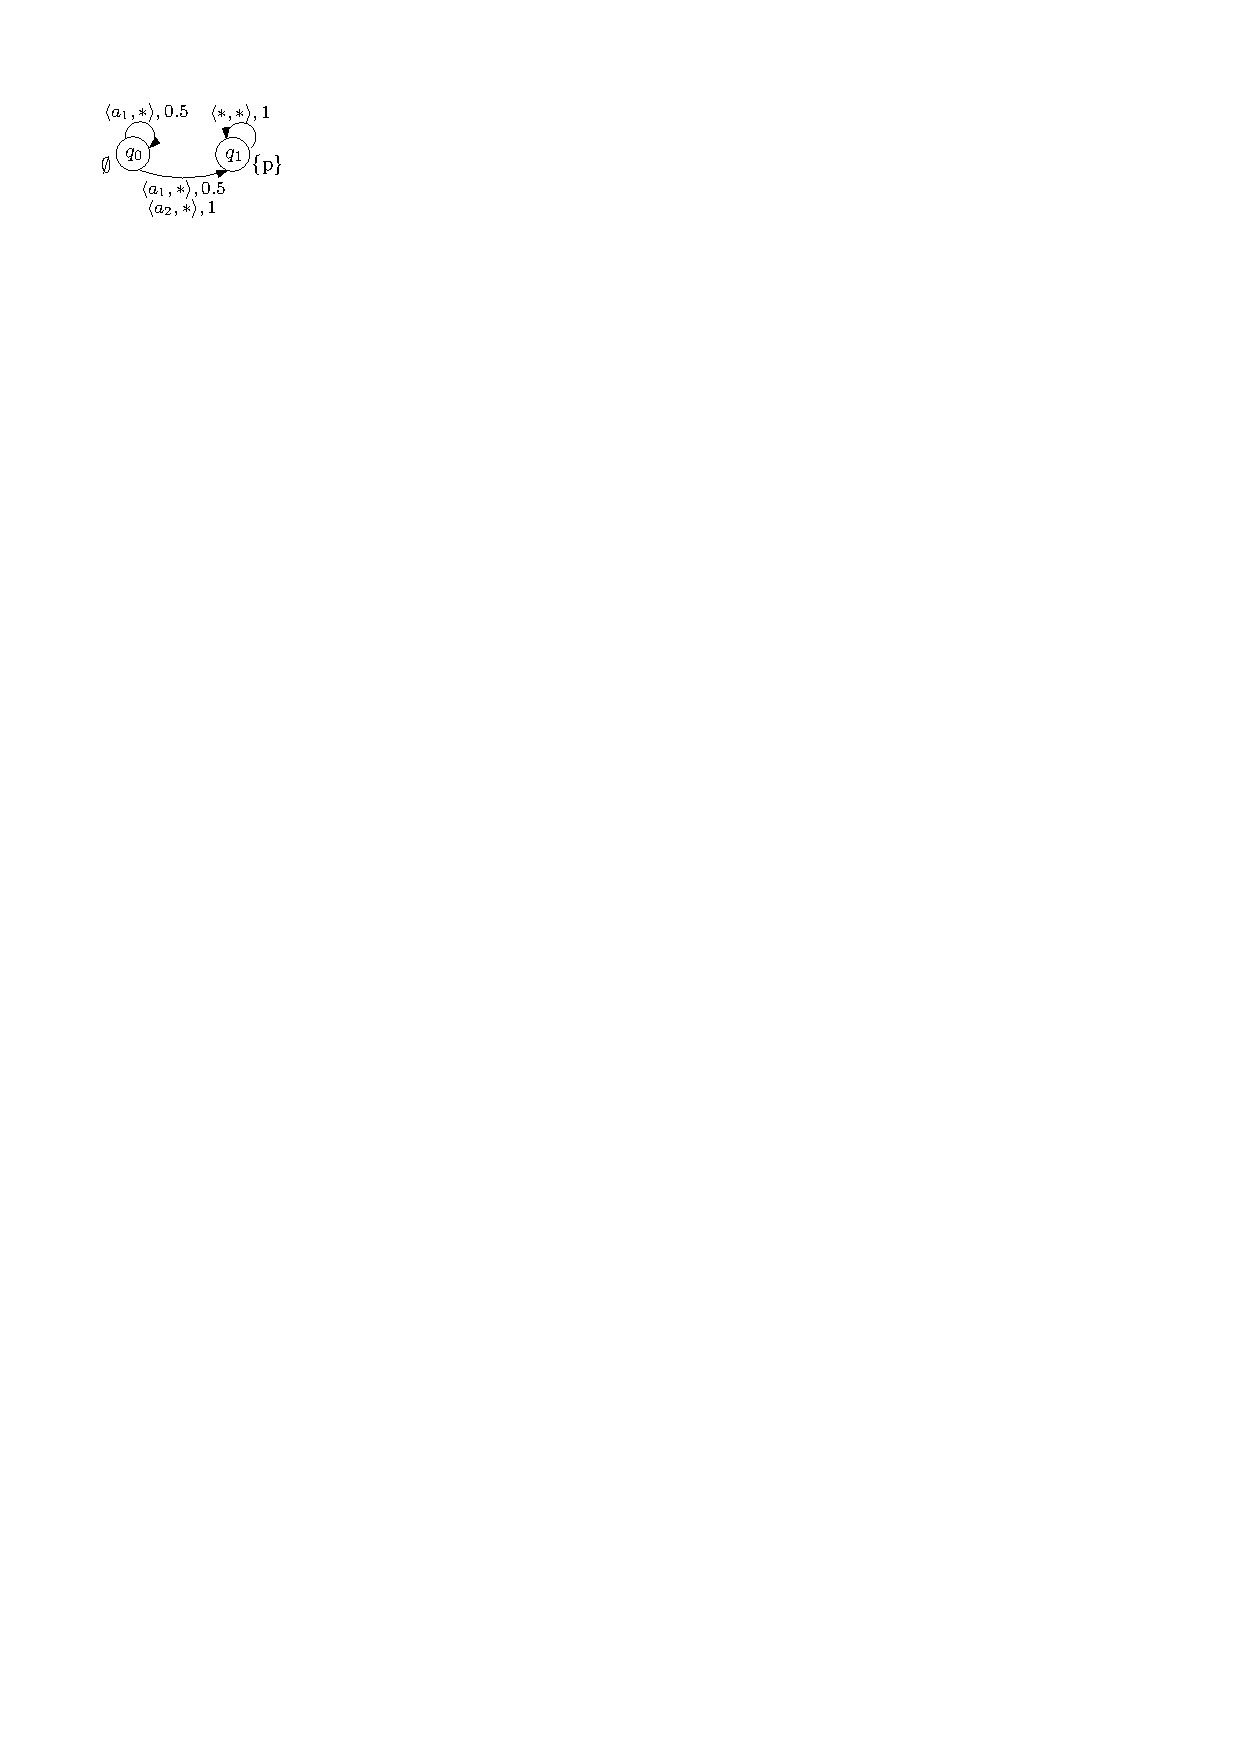
\includegraphics[width=0.18\textwidth]{figure//fig-example1}\\
  \caption{Example for memoryless property on \pamc, where $*\in\{a_1,a_2\}$.}\label{fig-example1}
\end{figure}

\begin{example}
Let us the pCGS $\calM=(\{1,2\},\{a_1,a_2\},\{q_0,q_1\}, \delta,\lambda, q_0)$ as shown in Figure \ref{fig-example1}, where for every $*\in\{a_1,a_2\}$,
\begin{itemize}
\item $\delta(q_0,\langle a_1,*\rangle, q_0)=0.5$ and $\delta(q_0,\langle a_1,*\rangle, q_1)=0.5$,
\item $\delta(q_0,\langle a_2,*\rangle, q_1)=1$,
\item $\delta(q_1,\dec,q_1)=1$ for every $\dec\in \{a_1,a_2\}^2$,
\item $\lambda(p)=\{q_1\}$.
\end{itemize}

Consider the closed \pamc state formula $\phi=\opA{\{1\}}^{\geq 0.5}\opX(\neg p \wedge \opX p)$ which states that
agent $1$ has a strategy such that whatever agent $2$ does, the probability to achieve the goal $\opX(\neg p \wedge \opX p)$
is no less than $0.5$. It is easy to see that there is no memoryless strategy for agent $1$ to achieve the goal, i.e.,
$\semantics{\phi}_\calM^r=\emptyset$. While $\semantics{\phi}_\calM^R=\{q_0\}$, as agent $1$ can use the strategy $\upsilon_{\{1\}}$
such that $\upsilon_{\{1\}}(q_0)(a_1)=1$ and $\upsilon_{\{1\}}(q_0q_0)(a_2)=1$.
\end{example}

\subsection{Randomized vs. Deterministic}
\begin{theorem}\label{thm-p2d}
Given a closed \pamc state formula $\phi$, let $\semantics{\phi}_\calM^p$ and $\semantics{\phi}_\calM^d$ respectively denote the set of states
satisfying $\phi$ under randomized and deterministic settings. Then,
$\semantics{\phi}_\calM^p=\semantics{\phi}_\calM^d$ under memoryful setting.
\end{theorem}
\begin{proof}
The proof is straightforward by induction on the structure of $\phi$.
We only need to consider principal formulae of the form $\opA{A}^{\sim c}\psi$ and $\opUA{A}^{\sim c}\psi$.
The proof for the case $\opA{A}^{\sim c}\psi$ follows from
Theorem \ref{thm-ltl2pa} and Lemma \ref{lemma-mc2spg}, while $\opUA{A}^{\sim c}\psi$
can be proved by switching players in the stochastic parity game.
\end{proof}

Let \pamc$^=$ be the logic by setting $\sim\in\{\geq,>,=\}$ in the \pamc.
Then, Theorem \ref{thm-p2d} will not hold for \pamc$^=$. We show this by the following example.




\begin{example}
Let us consider the pCGS
$\calM=(\{1,2\},\{a_1,a_2\},\{q_0,q_1\}, \delta,\lambda)$ as shown in Figure \ref{fig-example1} and the closed \pamc$^=$ state formula $\phi=\opA{\{1\}}\opX^{=0.75} p$.

In randomized setting, agent $1$ has a strategy $\upsilon_{\{1\}}$ such that for all strategies $\upsilon_{\{2\}}$ of agent $2$, $\Prb_{q_0}^{\upsilon_{\{1\}},\upsilon_{\{2\}}}(\{\rho\in \calP_{q_0}^{\upsilon_{\{1\}}, \upsilon_{\{2\}}}\mid \rho_1\in\semantics{p}_\calM^\xi\})=0.75$, where
$\upsilon_{\{1\}}(\pi)(a_1)=0.5$ and $\upsilon_{\{1\}}(\pi)(a_2)=0.5$. Therefore $q_0\in\semantics{p}_\calM^\xi$.
While, in deterministic setting, it is easy to see that $q_0\not\in\semantics{p}_\calM^\xi$.
\end{example}



\begin{figure}[h]
  \centering
  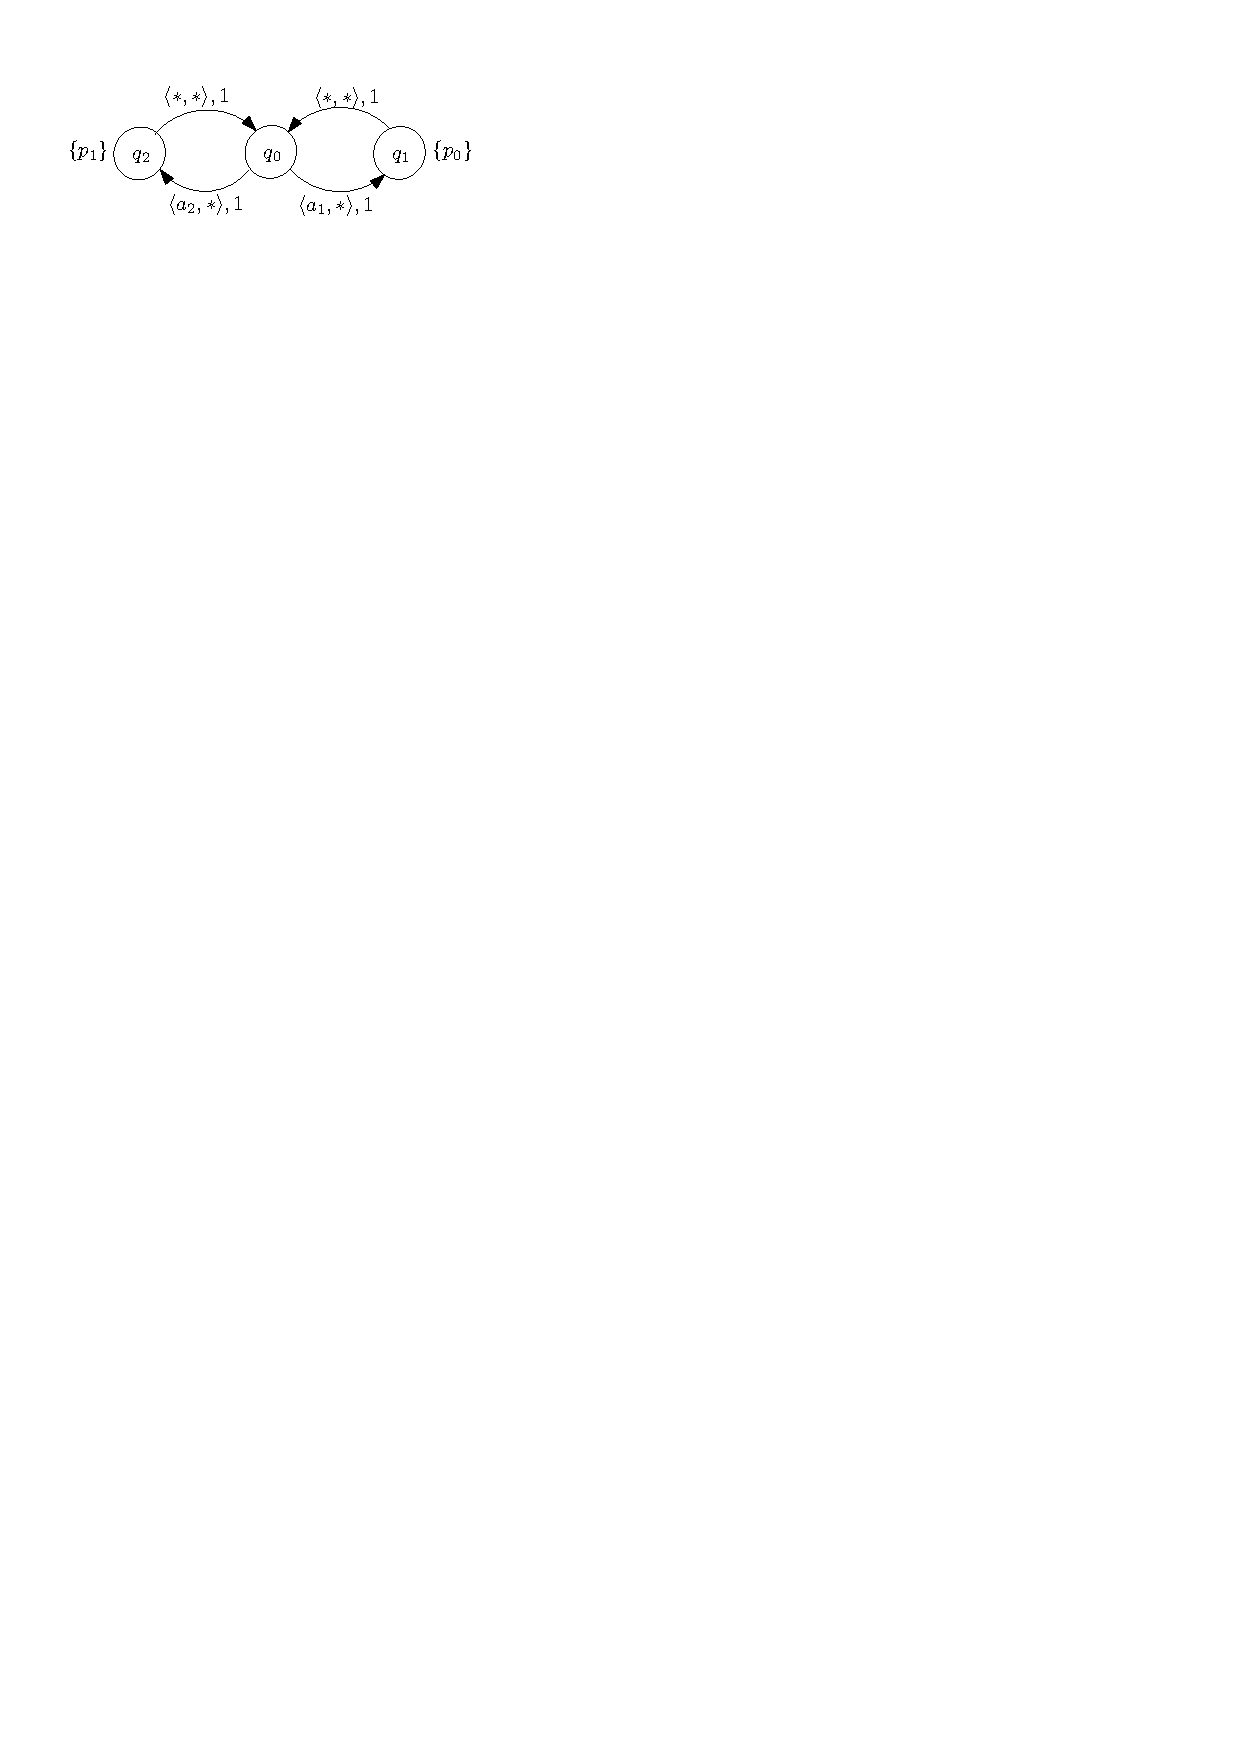
\includegraphics[width=0.35\textwidth]{figure//fig-example2}\\
  \caption{Example for determinacy, where $*\in\{a_1,a_2\}$.}\label{fig-example2}
\end{figure}


Under memoryless setting, \pamc does not have determinacy property as shown by the following example.
\begin{example}
Let us consider the pCGS
$\calM=(\{1,2\},\{a_1,a_2\},\{q_0,q_1,q_3\}, \delta,\lambda)$ as shown in Figure  \ref{fig-example2}
and the closed \pamc state formula $\phi=\opA{\{1\}}^{>0} (\mu_p Z. p_1 \wedge \mu_p Y. p_0)$.

Under randomized memoryless setting,  $q_0\in\semantics{\phi}_\calM^\xi$, while $q_0\not\in\semantics{\phi}_\calM^\xi$ under deterministic memoryless setting.
\end{example}

\end{document}
